\section{Mapping/Scheduling Exercice}

This exercise talks about improving the execution time of an application by changing the Scheduling and the Mapping of the tasks.

\subsection{New schedule}

As regarding the data dependencies, this schedule has been created to have the minimal length.

\bigskip

\begin{figure}[h!]
  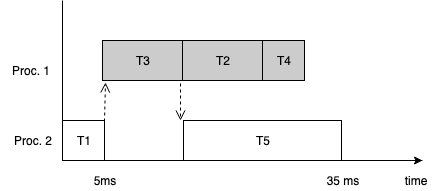
\includegraphics[width=\textwidth]{Ass3_1.png}
  \caption{New schedule}
  \label{fig:sys}
\end{figure}

By changing the schedule without changing the mapping, the goal is to find the best scheduling to avoid the wast of time.
The task T3 is required to allow the execution of T5 which is the longest task. T5 doesn't require T2 and T4, so T3 has to be before T2 to avoid that waste of time.

\newpage\subsection{New mapping}

This new schedule has been constructed by changing the mapping of tasks to processors. 

\bigskip

\begin{figure}[h!]
  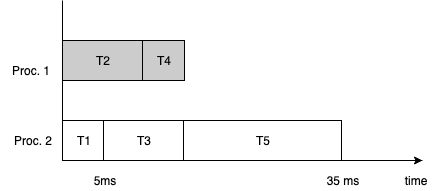
\includegraphics[width=\textwidth]{Ass3_2.png}
  \caption{New mapping}
  \label{fig:sys}
\end{figure}


By changing the mapping, the goal is to condense the tasks as much as possible. 
The tasks T1, T3, and T5 are dependent on each other and they need to be ordered like that. So a single processor can handle those different tasks. 
In the second hand, the tasks T2 and T4 can be run by another processor at the same time as T1, T2, and T5.
